\documentclass[1p]{elsarticle_modified}
%\bibliographystyle{elsarticle-num}

%\usepackage[colorlinks]{hyperref}
%\usepackage{abbrmath_seonhwa} %\Abb, \Ascr, \Acal ,\Abf, \Afrak
\usepackage{amsfonts}
\usepackage{amssymb}
\usepackage{amsmath}
\usepackage{amsthm}
\usepackage{scalefnt}
\usepackage{amsbsy}
\usepackage{kotex}
\usepackage{caption}
\usepackage{subfig}
\usepackage{color}
\usepackage{graphicx}
\usepackage{xcolor} %% white, black, red, green, blue, cyan, magenta, yellow
\usepackage{float}
\usepackage{setspace}
\usepackage{hyperref}

\usepackage{tikz}
\usetikzlibrary{arrows}

\usepackage{multirow}
\usepackage{array} % fixed length table
\usepackage{hhline}

%%%%%%%%%%%%%%%%%%%%%
\makeatletter
\renewcommand*\env@matrix[1][\arraystretch]{%
	\edef\arraystretch{#1}%
	\hskip -\arraycolsep
	\let\@ifnextchar\new@ifnextchar
	\array{*\c@MaxMatrixCols c}}
\makeatother %https://tex.stackexchange.com/questions/14071/how-can-i-increase-the-line-spacing-in-a-matrix
%%%%%%%%%%%%%%%

\usepackage[normalem]{ulem}

\newcommand{\msout}[1]{\ifmmode\text{\sout{\ensuremath{#1}}}\else\sout{#1}\fi}
%SOURCE: \msout is \stkout macro in https://tex.stackexchange.com/questions/20609/strikeout-in-math-mode

\newcommand{\cancel}[1]{
	\ifmmode
	{\color{red}\msout{#1}}
	\else
	{\color{red}\sout{#1}}
	\fi
}

\newcommand{\add}[1]{
	{\color{blue}\uwave{#1}}
}

\newcommand{\replace}[2]{
	\ifmmode
	{\color{red}\msout{#1}}{\color{blue}\uwave{#2}}
	\else
	{\color{red}\sout{#1}}{\color{blue}\uwave{#2}}
	\fi
}

\newcommand{\Sol}{\mathcal{S}} %segment
\newcommand{\D}{D} %diagram
\newcommand{\A}{\mathcal{A}} %arc


%%%%%%%%%%%%%%%%%%%%%%%%%%%%%5 test

\def\sl{\operatorname{\textup{SL}}(2,\Cbb)}
\def\psl{\operatorname{\textup{PSL}}(2,\Cbb)}
\def\quan{\mkern 1mu \triangleright \mkern 1mu}

\theoremstyle{definition}
\newtheorem{thm}{Theorem}[section]
\newtheorem{prop}[thm]{Proposition}
\newtheorem{lem}[thm]{Lemma}
\newtheorem{ques}[thm]{Question}
\newtheorem{cor}[thm]{Corollary}
\newtheorem{defn}[thm]{Definition}
\newtheorem{exam}[thm]{Example}
\newtheorem{rmk}[thm]{Remark}
\newtheorem{alg}[thm]{Algorithm}

\newcommand{\I}{\sqrt{-1}}
\begin{document}

%\begin{frontmatter}
%
%\title{Boundary parabolic representations of knots up to 8 crossings}
%
%%% Group authors per affiliation:
%\author{Yunhi Cho} 
%\address{Department of Mathematics, University of Seoul, Seoul, Korea}
%\ead{yhcho@uos.ac.kr}
%
%
%\author{Seonhwa Kim} %\fnref{s_kim}}
%\address{Center for Geometry and Physics, Institute for Basic Science, Pohang, 37673, Korea}
%\ead{ryeona17@ibs.re.kr}
%
%\author{Hyuk Kim}
%\address{Department of Mathematical Sciences, Seoul National University, Seoul 08826, Korea}
%\ead{hyukkim@snu.ac.kr}
%
%\author{Seokbeom Yoon}
%\address{Department of Mathematical Sciences, Seoul National University, Seoul, 08826,  Korea}
%\ead{sbyoon15@snu.ac.kr}
%
%\begin{abstract}
%We find all boundary parabolic representation of knots up to 8 crossings.
%
%\end{abstract}
%\begin{keyword}
%    \MSC[2010] 57M25 
%\end{keyword}
%
%\end{frontmatter}

%\linenumbers
%\tableofcontents
%
\newcommand\colored[1]{\textcolor{white}{\rule[-0.35ex]{0.8em}{1.4ex}}\kern-0.8em\color{red} #1}%
%\newcommand\colored[1]{\textcolor{white}{ #1}\kern-2.17ex	\textcolor{white}{ #1}\kern-1.81ex	\textcolor{white}{ #1}\kern-2.15ex\color{red}#1	}

{\Large $\underline{12a_{0155}~(K12a_{0155})}$}

\setlength{\tabcolsep}{10pt}
\renewcommand{\arraystretch}{1.6}
\vspace{1cm}\begin{tabular}{m{100pt}>{\centering\arraybackslash}m{274pt}}
\multirow{5}{120pt}{
	\centering
	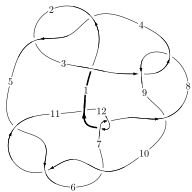
\includegraphics[width=112pt]{../../../GIT/diagram.site/Diagrams/png/956_12a_0155.png}\\
\ \ \ A knot diagram\footnotemark}&
\allowdisplaybreaks
\textbf{Linearized knot diagam} \\
\cline{2-2}
 &
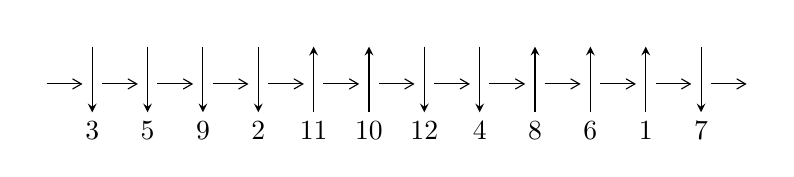
\begin{tikzpicture}[x=20pt, y=17pt]
	% nodes
	\node (C0) at (0, 0) {};
	\node (C1) at (1, 0) {};
	\node (C1U) at (1, +1) {};
	\node (C1D) at (1, -1) {3};

	\node (C2) at (2, 0) {};
	\node (C2U) at (2, +1) {};
	\node (C2D) at (2, -1) {5};

	\node (C3) at (3, 0) {};
	\node (C3U) at (3, +1) {};
	\node (C3D) at (3, -1) {9};

	\node (C4) at (4, 0) {};
	\node (C4U) at (4, +1) {};
	\node (C4D) at (4, -1) {2};

	\node (C5) at (5, 0) {};
	\node (C5U) at (5, +1) {};
	\node (C5D) at (5, -1) {11};

	\node (C6) at (6, 0) {};
	\node (C6U) at (6, +1) {};
	\node (C6D) at (6, -1) {10};

	\node (C7) at (7, 0) {};
	\node (C7U) at (7, +1) {};
	\node (C7D) at (7, -1) {12};

	\node (C8) at (8, 0) {};
	\node (C8U) at (8, +1) {};
	\node (C8D) at (8, -1) {4};

	\node (C9) at (9, 0) {};
	\node (C9U) at (9, +1) {};
	\node (C9D) at (9, -1) {8};

	\node (C10) at (10, 0) {};
	\node (C10U) at (10, +1) {};
	\node (C10D) at (10, -1) {6};

	\node (C11) at (11, 0) {};
	\node (C11U) at (11, +1) {};
	\node (C11D) at (11, -1) {1};

	\node (C12) at (12, 0) {};
	\node (C12U) at (12, +1) {};
	\node (C12D) at (12, -1) {7};
	\node (C13) at (13, 0) {};

	% arrows
	\draw[->,>={angle 60}]
	(C0) edge (C1) (C1) edge (C2) (C2) edge (C3) (C3) edge (C4) (C4) edge (C5) (C5) edge (C6) (C6) edge (C7) (C7) edge (C8) (C8) edge (C9) (C9) edge (C10) (C10) edge (C11) (C11) edge (C12) (C12) edge (C13) ;	\draw[->,>=stealth]
	(C1U) edge (C1D) (C2U) edge (C2D) (C3U) edge (C3D) (C4U) edge (C4D) (C5D) edge (C5U) (C6D) edge (C6U) (C7U) edge (C7D) (C8U) edge (C8D) (C9D) edge (C9U) (C10D) edge (C10U) (C11D) edge (C11U) (C12U) edge (C12D) ;
	\end{tikzpicture} \\
\hhline{~~} \\& 
\textbf{Solving Sequence} \\ \cline{2-2} 
 &
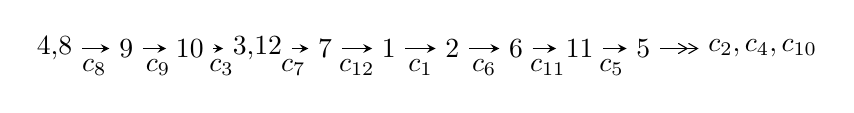
\begin{tikzpicture}[x=23pt, y=7pt]
	% node
	\node (A0) at (-1/8, 0) {4,8};
	\node (A1) at (1, 0) {9};
	\node (A2) at (2, 0) {10};
	\node (A3) at (49/16, 0) {3,12};
	\node (A4) at (33/8, 0) {7};
	\node (A5) at (41/8, 0) {1};
	\node (A6) at (49/8, 0) {2};
	\node (A7) at (57/8, 0) {6};
	\node (A8) at (65/8, 0) {11};
	\node (A9) at (73/8, 0) {5};
	\node (C1) at (1/2, -1) {$c_{8}$};
	\node (C2) at (3/2, -1) {$c_{9}$};
	\node (C3) at (5/2, -1) {$c_{3}$};
	\node (C4) at (29/8, -1) {$c_{7}$};
	\node (C5) at (37/8, -1) {$c_{12}$};
	\node (C6) at (45/8, -1) {$c_{1}$};
	\node (C7) at (53/8, -1) {$c_{6}$};
	\node (C8) at (61/8, -1) {$c_{11}$};
	\node (C9) at (69/8, -1) {$c_{5}$};
	\node (A10) at (11, 0) {$c_{2},c_{4},c_{10}$};

	% edge
	\draw[->,>=stealth]	
	(A0) edge (A1) (A1) edge (A2) (A2) edge (A3) (A3) edge (A4) (A4) edge (A5) (A5) edge (A6) (A6) edge (A7) (A7) edge (A8) (A8) edge (A9) ;
	\draw[->>,>={angle 60}]	
	(A9) edge (A10);
\end{tikzpicture} \\ 

\end{tabular} \\

\footnotetext{
The image of knot diagram is generated by the software ``\textbf{Draw programme}" developed by Andrew Bartholomew(\url{http://www.layer8.co.uk/maths/draw/index.htm\#Running-draw}), where we modified some parts for our purpose(\url{https://github.com/CATsTAILs/LinksPainter}).
}\phantom \\ \newline 
\centering \textbf{Ideals for irreducible components\footnotemark of $X_{\text{par}}$} 
 
\begin{align*}
I^u_{1}&=\langle 
-2.07210\times10^{79} u^{73}-4.45872\times10^{79} u^{72}+\cdots+1.81105\times10^{80} b-5.45671\times10^{80},\\
\phantom{I^u_{1}}&\phantom{= \langle  }9.44926\times10^{78} u^{73}+1.37256\times10^{79} u^{72}+\cdots+6.03683\times10^{79} a+2.79535\times10^{80},\;u^{74}+2 u^{73}+\cdots+16 u+64\rangle \\
I^u_{2}&=\langle 
12 u^8 a^2-12 u^8+\cdots-283 a-196,\;2 u^8 a^2+5 u^8 a+\cdots+9 a-20,\\
\phantom{I^u_{2}}&\phantom{= \langle  }u^9- u^8+2 u^7- u^6+3 u^5- u^4+2 u^3+u+1\rangle \\
I^u_{3}&=\langle 
u^{11}+2 u^9+2 u^7- u^3+b,\;- u^{10}+u^9-3 u^8+2 u^7-5 u^6+2 u^5-4 u^4-2 u^2+a- u-1,\\
\phantom{I^u_{3}}&\phantom{= \langle  }u^{12}+3 u^{10}+5 u^8+4 u^6+2 u^4+u^2+1\rangle \\
\\
I^v_{1}&=\langle 
a,\;-2 v^3+3 v^2+4 b-8 v+3,\;2 v^4- v^3+5 v^2+v+1\rangle \\
\end{align*}
\raggedright * 4 irreducible components of $\dim_{\mathbb{C}}=0$, with total 117 representations.\\
\footnotetext{All coefficients of polynomials are rational numbers. But the coefficients are sometimes approximated in decimal forms when there is not enough margin.}
\newpage
\renewcommand{\arraystretch}{1}
\centering \section*{I. $I^u_{1}= \langle -2.07\times10^{79} u^{73}-4.46\times10^{79} u^{72}+\cdots+1.81\times10^{80} b-5.46\times10^{80},\;9.45\times10^{78} u^{73}+1.37\times10^{79} u^{72}+\cdots+6.04\times10^{79} a+2.80\times10^{80},\;u^{74}+2 u^{73}+\cdots+16 u+64 \rangle$}
\flushleft \textbf{(i) Arc colorings}\\
\begin{tabular}{m{7pt} m{180pt} m{7pt} m{180pt} }
\flushright $a_{4}=$&$\begin{pmatrix}0\\u\end{pmatrix}$ \\
\flushright $a_{8}=$&$\begin{pmatrix}1\\0\end{pmatrix}$ \\
\flushright $a_{9}=$&$\begin{pmatrix}1\\u^2\end{pmatrix}$ \\
\flushright $a_{10}=$&$\begin{pmatrix}u^2+1\\u^2\end{pmatrix}$ \\
\flushright $a_{3}=$&$\begin{pmatrix}u\\u^3+u\end{pmatrix}$ \\
\flushright $a_{12}=$&$\begin{pmatrix}-0.156527 u^{73}-0.227365 u^{72}+\cdots-9.44771 u-4.63049\\0.114414 u^{73}+0.246195 u^{72}+\cdots+18.2624 u+3.01301\end{pmatrix}$ \\
\flushright $a_{7}=$&$\begin{pmatrix}-0.0427323 u^{73}-0.0222590 u^{72}+\cdots-17.0843 u-2.73523\\0.0558199 u^{73}+0.00860331 u^{72}+\cdots+7.08355 u-20.4297\end{pmatrix}$ \\
\flushright $a_{1}=$&$\begin{pmatrix}-0.247663 u^{73}-0.406614 u^{72}+\cdots-47.8687 u-2.35262\\-0.0419160 u^{73}-0.134596 u^{72}+\cdots-19.1036 u-12.4163\end{pmatrix}$ \\
\flushright $a_{2}=$&$\begin{pmatrix}-0.200457 u^{73}-0.360919 u^{72}+\cdots-39.4697 u-7.35311\\0.00721908 u^{73}-0.0715981 u^{72}+\cdots-12.9464 u-14.2988\end{pmatrix}$ \\
\flushright $a_{6}=$&$\begin{pmatrix}-0.0796114 u^{73}-0.0728386 u^{72}+\cdots-15.9420 u+4.33996\\0.101084 u^{73}+0.0798881 u^{72}+\cdots+11.6620 u-23.1448\end{pmatrix}$ \\
\flushright $a_{11}=$&$\begin{pmatrix}-0.143338 u^{73}-0.243103 u^{72}+\cdots-20.1363 u+2.92790\\-0.144745 u^{73}-0.280896 u^{72}+\cdots-39.7884 u+8.31570\end{pmatrix}$ \\
\flushright $a_{5}=$&$\begin{pmatrix}-0.150768 u^{73}-0.223403 u^{72}+\cdots-14.3340 u+4.38601\\0.0968957 u^{73}+0.183211 u^{72}+\cdots+33.5347 u+6.73864\end{pmatrix}$\\&\end{tabular}
\flushleft \textbf{(ii) Obstruction class $= -1$}\\~\\
\flushleft \textbf{(iii) Cusp Shapes $= -0.801859 u^{73}-1.46138 u^{72}+\cdots-97.4961 u+28.5646$}\\~\\
\newpage\renewcommand{\arraystretch}{1}
\flushleft \textbf{(iv) u-Polynomials at the component}\newline \\
\begin{tabular}{m{50pt}|m{274pt}}
Crossings & \hspace{64pt}u-Polynomials at each crossing \\
\hline $$\begin{aligned}c_{1}\end{aligned}$$&$\begin{aligned}
&u^{74}+40 u^{73}+\cdots+177 u+16
\end{aligned}$\\
\hline $$\begin{aligned}c_{2},c_{4}\end{aligned}$$&$\begin{aligned}
&u^{74}-4 u^{73}+\cdots-35 u+4
\end{aligned}$\\
\hline $$\begin{aligned}c_{3},c_{8}\end{aligned}$$&$\begin{aligned}
&u^{74}+2 u^{73}+\cdots+16 u+64
\end{aligned}$\\
\hline $$\begin{aligned}c_{5},c_{6},c_{10}\end{aligned}$$&$\begin{aligned}
&u^{74}+2 u^{73}+\cdots+78 u+9
\end{aligned}$\\
\hline $$\begin{aligned}c_{7},c_{12}\end{aligned}$$&$\begin{aligned}
&u^{74}+2 u^{73}+\cdots+54 u+9
\end{aligned}$\\
\hline $$\begin{aligned}c_{9}\end{aligned}$$&$\begin{aligned}
&u^{74}-24 u^{73}+\cdots-103168 u+4096
\end{aligned}$\\
\hline $$\begin{aligned}c_{11}\end{aligned}$$&$\begin{aligned}
&u^{74}-26 u^{73}+\cdots-2880 u+81
\end{aligned}$\\
\hline
\end{tabular}\\~\\
\newpage\renewcommand{\arraystretch}{1}
\flushleft \textbf{(v) Riley Polynomials at the component}\newline \\
\begin{tabular}{m{50pt}|m{274pt}}
Crossings & \hspace{64pt}Riley Polynomials at each crossing \\
\hline $$\begin{aligned}c_{1}\end{aligned}$$&$\begin{aligned}
&y^{74}-8 y^{73}+\cdots-5953 y+256
\end{aligned}$\\
\hline $$\begin{aligned}c_{2},c_{4}\end{aligned}$$&$\begin{aligned}
&y^{74}-40 y^{73}+\cdots-177 y+16
\end{aligned}$\\
\hline $$\begin{aligned}c_{3},c_{8}\end{aligned}$$&$\begin{aligned}
&y^{74}+24 y^{73}+\cdots+103168 y+4096
\end{aligned}$\\
\hline $$\begin{aligned}c_{5},c_{6},c_{10}\end{aligned}$$&$\begin{aligned}
&y^{74}+82 y^{73}+\cdots-3456 y+81
\end{aligned}$\\
\hline $$\begin{aligned}c_{7},c_{12}\end{aligned}$$&$\begin{aligned}
&y^{74}+26 y^{73}+\cdots+2880 y+81
\end{aligned}$\\
\hline $$\begin{aligned}c_{9}\end{aligned}$$&$\begin{aligned}
&y^{74}+44 y^{73}+\cdots-654376960 y+16777216
\end{aligned}$\\
\hline $$\begin{aligned}c_{11}\end{aligned}$$&$\begin{aligned}
&y^{74}+58 y^{73}+\cdots+591300 y+6561
\end{aligned}$\\
\hline
\end{tabular}\\~\\
\newpage\flushleft \textbf{(vi) Complex Volumes and Cusp Shapes}
$$\begin{array}{c|c|c}  
\text{Solutions to }I^u_{1}& \I (\text{vol} + \sqrt{-1}CS) & \text{Cusp shape}\\
 \hline 
\begin{aligned}
u &= -1.016280 + 0.056443 I \\
a &= -0.846246 - 0.233543 I \\
b &= -0.641966 - 0.915109 I\end{aligned}
 & -4.55260 - 4.71728 I & -5.48750 + 5.97757 I \\ \hline\begin{aligned}
u &= -1.016280 - 0.056443 I \\
a &= -0.846246 + 0.233543 I \\
b &= -0.641966 + 0.915109 I\end{aligned}
 & -4.55260 + 4.71728 I & -5.48750 - 5.97757 I \\ \hline\begin{aligned}
u &= \phantom{-}0.715978 + 0.749309 I \\
a &= -1.009060 + 0.512831 I \\
b &= -0.819433 + 1.097530 I\end{aligned}
 & -10.62080 + 2.16848 I & -8.29410 + 0. I\phantom{ +0.000000I} \\ \hline\begin{aligned}
u &= \phantom{-}0.715978 - 0.749309 I \\
a &= -1.009060 - 0.512831 I \\
b &= -0.819433 - 1.097530 I\end{aligned}
 & -10.62080 - 2.16848 I & -8.29410 + 0. I\phantom{ +0.000000I} \\ \hline\begin{aligned}
u &= \phantom{-}1.018120 + 0.241002 I \\
a &= -0.883835 - 0.063210 I \\
b &= -0.634326 - 0.779842 I\end{aligned}
 & -4.97717 - 0.27862 I & -6.77921 + 0. I\phantom{ +0.000000I} \\ \hline\begin{aligned}
u &= \phantom{-}1.018120 - 0.241002 I \\
a &= -0.883835 + 0.063210 I \\
b &= -0.634326 + 0.779842 I\end{aligned}
 & -4.97717 + 0.27862 I & -6.77921 + 0. I\phantom{ +0.000000I} \\ \hline\begin{aligned}
u &= \phantom{-}0.101684 + 0.941180 I \\
a &= -0.96039 + 1.37103 I \\
b &= \phantom{-}0.668786 - 0.848557 I\end{aligned}
 & -6.34170 + 2.58749 I & -5.26885 - 2.40308 I \\ \hline\begin{aligned}
u &= \phantom{-}0.101684 - 0.941180 I \\
a &= -0.96039 - 1.37103 I \\
b &= \phantom{-}0.668786 + 0.848557 I\end{aligned}
 & -6.34170 - 2.58749 I & -5.26885 + 2.40308 I \\ \hline\begin{aligned}
u &= \phantom{-}0.702951 + 0.605779 I \\
a &= \phantom{-}1.083580 - 0.777415 I \\
b &= \phantom{-}0.577935 - 0.892143 I\end{aligned}
 & -0.36424 + 2.16926 I & -1.33400 - 2.94106 I \\ \hline\begin{aligned}
u &= \phantom{-}0.702951 - 0.605779 I \\
a &= \phantom{-}1.083580 + 0.777415 I \\
b &= \phantom{-}0.577935 + 0.892143 I\end{aligned}
 & -0.36424 - 2.16926 I & -1.33400 + 2.94106 I\\
 \hline 
 \end{array}$$\newpage$$\begin{array}{c|c|c}  
\text{Solutions to }I^u_{1}& \I (\text{vol} + \sqrt{-1}CS) & \text{Cusp shape}\\
 \hline 
\begin{aligned}
u &= \phantom{-}0.455877 + 0.982311 I \\
a &= \phantom{-}0.549167 + 0.442923 I \\
b &= \phantom{-}0.532038 + 0.022585 I\end{aligned}
 & -1.99851 - 5.40155 I & \phantom{-0.000000 } 0 \\ \hline\begin{aligned}
u &= \phantom{-}0.455877 - 0.982311 I \\
a &= \phantom{-}0.549167 - 0.442923 I \\
b &= \phantom{-}0.532038 - 0.022585 I\end{aligned}
 & -1.99851 + 5.40155 I & \phantom{-0.000000 } 0 \\ \hline\begin{aligned}
u &= -0.688565 + 0.844832 I \\
a &= -2.45152 - 0.54418 I \\
b &= -0.623313 + 0.954050 I\end{aligned}
 & -3.63561 + 3.57244 I & \phantom{-0.000000 } 0 \\ \hline\begin{aligned}
u &= -0.688565 - 0.844832 I \\
a &= -2.45152 + 0.54418 I \\
b &= -0.623313 - 0.954050 I\end{aligned}
 & -3.63561 - 3.57244 I & \phantom{-0.000000 } 0 \\ \hline\begin{aligned}
u &= -0.922080 + 0.581194 I \\
a &= -0.902921 - 0.473277 I \\
b &= -0.730349 - 1.085650 I\end{aligned}
 & -6.70976 - 5.72717 I & \phantom{-0.000000 } 0 \\ \hline\begin{aligned}
u &= -0.922080 - 0.581194 I \\
a &= -0.902921 + 0.473277 I \\
b &= -0.730349 + 1.085650 I\end{aligned}
 & -6.70976 + 5.72717 I & \phantom{-0.000000 } 0 \\ \hline\begin{aligned}
u &= \phantom{-}0.400961 + 1.025910 I \\
a &= \phantom{-}0.513025 - 0.645985 I \\
b &= -0.156641 + 1.061890 I\end{aligned}
 & \phantom{-}3.87862 - 1.01189 I & \phantom{-0.000000 } 0 \\ \hline\begin{aligned}
u &= \phantom{-}0.400961 - 1.025910 I \\
a &= \phantom{-}0.513025 + 0.645985 I \\
b &= -0.156641 - 1.061890 I\end{aligned}
 & \phantom{-}3.87862 + 1.01189 I & \phantom{-0.000000 } 0 \\ \hline\begin{aligned}
u &= -0.039055 + 1.116760 I \\
a &= -0.491876 - 1.057740 I \\
b &= -0.338560 + 1.089190 I\end{aligned}
 & \phantom{-}5.21780 + 1.15055 I & \phantom{-0.000000 } 0 \\ \hline\begin{aligned}
u &= -0.039055 - 1.116760 I \\
a &= -0.491876 + 1.057740 I \\
b &= -0.338560 - 1.089190 I\end{aligned}
 & \phantom{-}5.21780 - 1.15055 I & \phantom{-0.000000 } 0\\
 \hline 
 \end{array}$$\newpage$$\begin{array}{c|c|c}  
\text{Solutions to }I^u_{1}& \I (\text{vol} + \sqrt{-1}CS) & \text{Cusp shape}\\
 \hline 
\begin{aligned}
u &= -0.686707 + 0.883279 I \\
a &= \phantom{-}1.136820 + 0.777943 I \\
b &= \phantom{-}0.710003 + 0.868137 I\end{aligned}
 & -3.51612 + 1.72512 I & \phantom{-0.000000 } 0 \\ \hline\begin{aligned}
u &= -0.686707 - 0.883279 I \\
a &= \phantom{-}1.136820 - 0.777943 I \\
b &= \phantom{-}0.710003 - 0.868137 I\end{aligned}
 & -3.51612 - 1.72512 I & \phantom{-0.000000 } 0 \\ \hline\begin{aligned}
u &= -0.780808 + 0.406319 I \\
a &= \phantom{-}1.069120 - 0.412845 I \\
b &= \phantom{-}0.132045 - 0.962513 I\end{aligned}
 & -0.190732 - 0.765674 I & \phantom{-}0.883971 + 0.910639 I \\ \hline\begin{aligned}
u &= -0.780808 - 0.406319 I \\
a &= \phantom{-}1.069120 + 0.412845 I \\
b &= \phantom{-}0.132045 + 0.962513 I\end{aligned}
 & -0.190732 + 0.765674 I & \phantom{-}0.883971 - 0.910639 I \\ \hline\begin{aligned}
u &= \phantom{-}0.868207 + 0.709119 I \\
a &= -1.316090 + 0.047838 I \\
b &= -0.932909 - 0.593077 I\end{aligned}
 & -8.22620 - 0.36510 I & \phantom{-0.000000 } 0 \\ \hline\begin{aligned}
u &= \phantom{-}0.868207 - 0.709119 I \\
a &= -1.316090 - 0.047838 I \\
b &= -0.932909 + 0.593077 I\end{aligned}
 & -8.22620 + 0.36510 I & \phantom{-0.000000 } 0 \\ \hline\begin{aligned}
u &= -0.773522 + 0.832238 I \\
a &= -1.388560 + 0.057416 I \\
b &= -1.017760 + 0.654828 I\end{aligned}
 & -11.98240 + 4.46440 I & \phantom{-0.000000 } 0 \\ \hline\begin{aligned}
u &= -0.773522 - 0.832238 I \\
a &= -1.388560 - 0.057416 I \\
b &= -1.017760 - 0.654828 I\end{aligned}
 & -11.98240 - 4.46440 I & \phantom{-0.000000 } 0 \\ \hline\begin{aligned}
u &= -0.923574 + 0.692893 I \\
a &= \phantom{-}1.084650 + 0.825348 I \\
b &= \phantom{-}0.628177 + 0.990952 I\end{aligned}
 & -3.34148 - 6.33239 I & \phantom{-0.000000 } 0 \\ \hline\begin{aligned}
u &= -0.923574 - 0.692893 I \\
a &= \phantom{-}1.084650 - 0.825348 I \\
b &= \phantom{-}0.628177 - 0.990952 I\end{aligned}
 & -3.34148 + 6.33239 I & \phantom{-0.000000 } 0\\
 \hline 
 \end{array}$$\newpage$$\begin{array}{c|c|c}  
\text{Solutions to }I^u_{1}& \I (\text{vol} + \sqrt{-1}CS) & \text{Cusp shape}\\
 \hline 
\begin{aligned}
u &= \phantom{-}0.643430 + 0.541266 I \\
a &= \phantom{-}0.11958 + 1.53542 I \\
b &= -0.096809 + 0.216360 I\end{aligned}
 & -3.46513 + 1.05609 I & -11.55620 - 0.54689 I \\ \hline\begin{aligned}
u &= \phantom{-}0.643430 - 0.541266 I \\
a &= \phantom{-}0.11958 - 1.53542 I \\
b &= -0.096809 - 0.216360 I\end{aligned}
 & -3.46513 - 1.05609 I & -11.55620 + 0.54689 I \\ \hline\begin{aligned}
u &= \phantom{-}0.251058 + 1.133180 I \\
a &= -1.05747 + 0.95104 I \\
b &= -0.431302 - 1.095140 I\end{aligned}
 & \phantom{-}4.59696 - 6.09538 I & \phantom{-0.000000 } 0 \\ \hline\begin{aligned}
u &= \phantom{-}0.251058 - 1.133180 I \\
a &= -1.05747 - 0.95104 I \\
b &= -0.431302 + 1.095140 I\end{aligned}
 & \phantom{-}4.59696 + 6.09538 I & \phantom{-0.000000 } 0 \\ \hline\begin{aligned}
u &= \phantom{-}0.680178 + 0.965059 I \\
a &= \phantom{-}2.06174 - 1.01173 I \\
b &= \phantom{-}0.733930 + 1.124350 I\end{aligned}
 & -9.95050 - 7.53602 I & \phantom{-0.000000 } 0 \\ \hline\begin{aligned}
u &= \phantom{-}0.680178 - 0.965059 I \\
a &= \phantom{-}2.06174 + 1.01173 I \\
b &= \phantom{-}0.733930 - 1.124350 I\end{aligned}
 & -9.95050 + 7.53602 I & \phantom{-0.000000 } 0 \\ \hline\begin{aligned}
u &= -0.760147 + 0.919939 I \\
a &= \phantom{-}0.363285 + 1.114770 I \\
b &= \phantom{-}0.972224 + 0.550351 I\end{aligned}
 & -11.71740 + 1.32226 I & \phantom{-0.000000 } 0 \\ \hline\begin{aligned}
u &= -0.760147 - 0.919939 I \\
a &= \phantom{-}0.363285 - 1.114770 I \\
b &= \phantom{-}0.972224 - 0.550351 I\end{aligned}
 & -11.71740 - 1.32226 I & \phantom{-0.000000 } 0 \\ \hline\begin{aligned}
u &= \phantom{-}0.785310 + 0.041797 I \\
a &= \phantom{-}1.032650 - 0.688989 I \\
b &= \phantom{-}0.336202 - 0.946046 I\end{aligned}
 & \phantom{-}0.75306 + 2.46584 I & \phantom{-}1.27659 - 6.33944 I \\ \hline\begin{aligned}
u &= \phantom{-}0.785310 - 0.041797 I \\
a &= \phantom{-}1.032650 + 0.688989 I \\
b &= \phantom{-}0.336202 + 0.946046 I\end{aligned}
 & \phantom{-}0.75306 - 2.46584 I & \phantom{-}1.27659 + 6.33944 I\\
 \hline 
 \end{array}$$\newpage$$\begin{array}{c|c|c}  
\text{Solutions to }I^u_{1}& \I (\text{vol} + \sqrt{-1}CS) & \text{Cusp shape}\\
 \hline 
\begin{aligned}
u &= \phantom{-}0.669060 + 1.015260 I \\
a &= -2.02541 + 0.47750 I \\
b &= -0.619534 - 1.034680 I\end{aligned}
 & \phantom{-}0.81052 - 7.48437 I & \phantom{-0.000000 } 0 \\ \hline\begin{aligned}
u &= \phantom{-}0.669060 - 1.015260 I \\
a &= -2.02541 - 0.47750 I \\
b &= -0.619534 + 1.034680 I\end{aligned}
 & \phantom{-}0.81052 + 7.48437 I & \phantom{-0.000000 } 0 \\ \hline\begin{aligned}
u &= -0.602047 + 1.071410 I \\
a &= \phantom{-}0.540817 + 0.305119 I \\
b &= -0.091548 - 1.090250 I\end{aligned}
 & \phantom{-}1.71998 + 5.88464 I & \phantom{-0.000000 } 0 \\ \hline\begin{aligned}
u &= -0.602047 - 1.071410 I \\
a &= \phantom{-}0.540817 - 0.305119 I \\
b &= -0.091548 + 1.090250 I\end{aligned}
 & \phantom{-}1.71998 - 5.88464 I & \phantom{-0.000000 } 0 \\ \hline\begin{aligned}
u &= -0.962055 + 0.769007 I \\
a &= -1.407370 - 0.115629 I \\
b &= -0.982890 + 0.515422 I\end{aligned}
 & -11.46460 - 4.27058 I & \phantom{-0.000000 } 0 \\ \hline\begin{aligned}
u &= -0.962055 - 0.769007 I \\
a &= -1.407370 + 0.115629 I \\
b &= -0.982890 - 0.515422 I\end{aligned}
 & -11.46460 + 4.27058 I & \phantom{-0.000000 } 0 \\ \hline\begin{aligned}
u &= \phantom{-}1.018000 + 0.713154 I \\
a &= -0.877403 + 0.545175 I \\
b &= -0.723054 + 1.145040 I\end{aligned}
 & -9.5271 + 10.4754 I & \phantom{-0.000000 } 0 \\ \hline\begin{aligned}
u &= \phantom{-}1.018000 - 0.713154 I \\
a &= -0.877403 - 0.545175 I \\
b &= -0.723054 - 1.145040 I\end{aligned}
 & -9.5271 - 10.4754 I & \phantom{-0.000000 } 0 \\ \hline\begin{aligned}
u &= -0.322053 + 1.215640 I \\
a &= -0.289638 - 0.522660 I \\
b &= \phantom{-}0.510459 + 0.750000 I\end{aligned}
 & -0.063900 - 0.320410 I & \phantom{-0.000000 } 0 \\ \hline\begin{aligned}
u &= -0.322053 - 1.215640 I \\
a &= -0.289638 + 0.522660 I \\
b &= \phantom{-}0.510459 - 0.750000 I\end{aligned}
 & -0.063900 + 0.320410 I & \phantom{-0.000000 } 0\\
 \hline 
 \end{array}$$\newpage$$\begin{array}{c|c|c}  
\text{Solutions to }I^u_{1}& \I (\text{vol} + \sqrt{-1}CS) & \text{Cusp shape}\\
 \hline 
\begin{aligned}
u &= \phantom{-}0.757308 + 1.014150 I \\
a &= \phantom{-}0.521716 - 0.835498 I \\
b &= \phantom{-}0.980452 - 0.466162 I\end{aligned}
 & -7.29295 - 5.66257 I & \phantom{-0.000000 } 0 \\ \hline\begin{aligned}
u &= \phantom{-}0.757308 - 1.014150 I \\
a &= \phantom{-}0.521716 + 0.835498 I \\
b &= \phantom{-}0.980452 + 0.466162 I\end{aligned}
 & -7.29295 + 5.66257 I & \phantom{-0.000000 } 0 \\ \hline\begin{aligned}
u &= \phantom{-}0.141074 + 1.267450 I \\
a &= \phantom{-}0.314381 - 1.040930 I \\
b &= \phantom{-}0.549097 + 0.971551 I\end{aligned}
 & \phantom{-}0.71079 - 3.98529 I & \phantom{-0.000000 } 0 \\ \hline\begin{aligned}
u &= \phantom{-}0.141074 - 1.267450 I \\
a &= \phantom{-}0.314381 + 1.040930 I \\
b &= \phantom{-}0.549097 - 0.971551 I\end{aligned}
 & \phantom{-}0.71079 + 3.98529 I & \phantom{-0.000000 } 0 \\ \hline\begin{aligned}
u &= -0.257906 + 0.673206 I \\
a &= \phantom{-}0.875017 - 0.842641 I \\
b &= \phantom{-}0.362715 - 0.412513 I\end{aligned}
 & -0.25584 + 1.43316 I & -2.89373 - 4.25664 I \\ \hline\begin{aligned}
u &= -0.257906 - 0.673206 I \\
a &= \phantom{-}0.875017 + 0.842641 I \\
b &= \phantom{-}0.362715 + 0.412513 I\end{aligned}
 & -0.25584 - 1.43316 I & -2.89373 + 4.25664 I \\ \hline\begin{aligned}
u &= \phantom{-}0.512625 + 1.186330 I \\
a &= -0.180598 + 0.307148 I \\
b &= \phantom{-}0.462194 - 0.608975 I\end{aligned}
 & -1.73996 - 5.08791 I & \phantom{-0.000000 } 0 \\ \hline\begin{aligned}
u &= \phantom{-}0.512625 - 1.186330 I \\
a &= -0.180598 - 0.307148 I \\
b &= \phantom{-}0.462194 + 0.608975 I\end{aligned}
 & -1.73996 + 5.08791 I & \phantom{-0.000000 } 0 \\ \hline\begin{aligned}
u &= -0.766224 + 1.056700 I \\
a &= -2.02146 - 0.26151 I \\
b &= -0.666344 + 1.052100 I\end{aligned}
 & -2.19593 + 12.55800 I & \phantom{-0.000000 } 0 \\ \hline\begin{aligned}
u &= -0.766224 - 1.056700 I \\
a &= -2.02146 + 0.26151 I \\
b &= -0.666344 - 1.052100 I\end{aligned}
 & -2.19593 - 12.55800 I & \phantom{-0.000000 } 0\\
 \hline 
 \end{array}$$\newpage$$\begin{array}{c|c|c}  
\text{Solutions to }I^u_{1}& \I (\text{vol} + \sqrt{-1}CS) & \text{Cusp shape}\\
 \hline 
\begin{aligned}
u &= -0.334080 + 1.262000 I \\
a &= \phantom{-}0.739927 + 1.023500 I \\
b &= \phantom{-}0.574354 - 1.047070 I\end{aligned}
 & -0.23035 + 9.53465 I & \phantom{-0.000000 } 0 \\ \hline\begin{aligned}
u &= -0.334080 - 1.262000 I \\
a &= \phantom{-}0.739927 - 1.023500 I \\
b &= \phantom{-}0.574354 + 1.047070 I\end{aligned}
 & -0.23035 - 9.53465 I & \phantom{-0.000000 } 0 \\ \hline\begin{aligned}
u &= -0.726282 + 1.091930 I \\
a &= \phantom{-}1.77788 + 0.71191 I \\
b &= \phantom{-}0.700817 - 1.164010 I\end{aligned}
 & -5.15120 + 11.77850 I & \phantom{-0.000000 } 0 \\ \hline\begin{aligned}
u &= -0.726282 - 1.091930 I \\
a &= \phantom{-}1.77788 - 0.71191 I \\
b &= \phantom{-}0.700817 + 1.164010 I\end{aligned}
 & -5.15120 - 11.77850 I & \phantom{-0.000000 } 0 \\ \hline\begin{aligned}
u &= -0.817220 + 1.044540 I \\
a &= \phantom{-}0.714742 + 0.868490 I \\
b &= \phantom{-}1.041650 + 0.454586 I\end{aligned}
 & -10.5690 + 10.7948 I & \phantom{-0.000000 } 0 \\ \hline\begin{aligned}
u &= -0.817220 - 1.044540 I \\
a &= \phantom{-}0.714742 - 0.868490 I \\
b &= \phantom{-}1.041650 - 0.454586 I\end{aligned}
 & -10.5690 - 10.7948 I & \phantom{-0.000000 } 0 \\ \hline\begin{aligned}
u &= \phantom{-}0.810773 + 1.098430 I \\
a &= \phantom{-}1.85420 - 0.50706 I \\
b &= \phantom{-}0.716271 + 1.194250 I\end{aligned}
 & -8.2766 - 17.1352 I & \phantom{-0.000000 } 0 \\ \hline\begin{aligned}
u &= \phantom{-}0.810773 - 1.098430 I \\
a &= \phantom{-}1.85420 + 0.50706 I \\
b &= \phantom{-}0.716271 - 1.194250 I\end{aligned}
 & -8.2766 + 17.1352 I & \phantom{-0.000000 } 0 \\ \hline\begin{aligned}
u &= -0.189049 + 0.597095 I \\
a &= \phantom{-}2.34091 + 2.24975 I \\
b &= -0.233253 - 0.857584 I\end{aligned}
 & -0.892082 - 1.083450 I & \phantom{-}4.37786 - 0.74207 I \\ \hline\begin{aligned}
u &= -0.189049 - 0.597095 I \\
a &= \phantom{-}2.34091 - 2.24975 I \\
b &= -0.233253 + 0.857584 I\end{aligned}
 & -0.892082 + 1.083450 I & \phantom{-}4.37786 + 0.74207 I\\
 \hline 
 \end{array}$$\newpage$$\begin{array}{c|c|c}  
\text{Solutions to }I^u_{1}& \I (\text{vol} + \sqrt{-1}CS) & \text{Cusp shape}\\
 \hline 
\begin{aligned}
u &= -0.022832 + 0.605905 I \\
a &= \phantom{-}1.015490 - 0.770054 I \\
b &= \phantom{-}0.451799 - 0.569597 I\end{aligned}
 & -0.20066 + 1.45515 I & -0.46303 - 4.13714 I \\ \hline\begin{aligned}
u &= -0.022832 - 0.605905 I \\
a &= \phantom{-}1.015490 + 0.770054 I \\
b &= \phantom{-}0.451799 + 0.569597 I\end{aligned}
 & -0.20066 - 1.45515 I & -0.46303 + 4.13714 I \\ \hline\begin{aligned}
u &= \phantom{-}0.057884 + 0.497232 I \\
a &= -1.161350 - 0.318274 I \\
b &= -0.901151 - 0.915137 I\end{aligned}
 & -8.05648 - 3.30418 I & \phantom{-}5.21911 + 6.27707 I \\ \hline\begin{aligned}
u &= \phantom{-}0.057884 - 0.497232 I \\
a &= -1.161350 + 0.318274 I \\
b &= -0.901151 + 0.915137 I\end{aligned}
 & -8.05648 + 3.30418 I & \phantom{-}5.21911 - 6.27707 I\\
 \hline 
 \end{array}$$\newpage\newpage\renewcommand{\arraystretch}{1}
\centering \section*{II. $I^u_{2}= \langle 12 u^8 a^2-12 u^8+\cdots-283 a-196,\;2 u^8 a^2+5 u^8 a+\cdots+9 a-20,\;u^9- u^8+2 u^7- u^6+3 u^5- u^4+2 u^3+u+1 \rangle$}
\flushleft \textbf{(i) Arc colorings}\\
\begin{tabular}{m{7pt} m{180pt} m{7pt} m{180pt} }
\flushright $a_{4}=$&$\begin{pmatrix}0\\u\end{pmatrix}$ \\
\flushright $a_{8}=$&$\begin{pmatrix}1\\0\end{pmatrix}$ \\
\flushright $a_{9}=$&$\begin{pmatrix}1\\u^2\end{pmatrix}$ \\
\flushright $a_{10}=$&$\begin{pmatrix}u^2+1\\u^2\end{pmatrix}$ \\
\flushright $a_{3}=$&$\begin{pmatrix}u\\u^3+u\end{pmatrix}$ \\
\flushright $a_{12}=$&$\begin{pmatrix}a\\-0.0424028 a^{2} u^{8}+0.0424028 u^{8}+\cdots+a+0.692580\end{pmatrix}$ \\
\flushright $a_{7}=$&$\begin{pmatrix}0.0424028 a^{2} u^{8}-0.0424028 u^{8}+\cdots-0.307420 a^{2}+1.30742\\0.0424028 a^{2} u^{8}-0.0424028 u^{8}+\cdots-0.307420 a^{2}+1.30742\end{pmatrix}$ \\
\flushright $a_{1}=$&$\begin{pmatrix}u^2+1\\u^2\end{pmatrix}$ \\
\flushright $a_{2}=$&$\begin{pmatrix}u^6+u^4+2 u^2+1\\u^8+2 u^6+2 u^4+2 u^2\end{pmatrix}$ \\
\flushright $a_{6}=$&$\begin{pmatrix}0.0848057 a^{2} u^{8}-0.0848057 u^{8}+\cdots-0.614841 a^{2}+2.61484\\0.127208 a^{2} u^{8}-0.127208 u^{8}+\cdots-a+1.92226\end{pmatrix}$ \\
\flushright $a_{11}=$&$\begin{pmatrix}0.0424028 a^{2} u^{8}-0.0424028 u^{8}+\cdots+2 a-0.692580\\0.0424028 a^{2} u^{8}-0.0424028 u^{8}+\cdots+2 a+1.30742\end{pmatrix}$ \\
\flushright $a_{5}=$&$\begin{pmatrix}u^4+u^2+1\\u^4\end{pmatrix}$\\&\end{tabular}
\flushleft \textbf{(ii) Obstruction class $= -1$}\\~\\
\flushleft \textbf{(iii) Cusp Shapes $= 4 u^7-4 u^6+4 u^5-4 u^4+8 u^3-4 u^2-6$}\\~\\
\newpage\renewcommand{\arraystretch}{1}
\flushleft \textbf{(iv) u-Polynomials at the component}\newline \\
\begin{tabular}{m{50pt}|m{274pt}}
Crossings & \hspace{64pt}u-Polynomials at each crossing \\
\hline $$\begin{aligned}c_{1}\end{aligned}$$&$\begin{aligned}
&(u^9+5 u^8+12 u^7+15 u^6+9 u^5- u^4-4 u^3-2 u^2+u+1)^3
\end{aligned}$\\
\hline $$\begin{aligned}c_{2},c_{4}\end{aligned}$$&$\begin{aligned}
&(u^9- u^8-2 u^7+3 u^6+u^5-3 u^4+2 u^3- u+1)^3
\end{aligned}$\\
\hline $$\begin{aligned}c_{3},c_{8}\end{aligned}$$&$\begin{aligned}
&(u^9- u^8+2 u^7- u^6+3 u^5- u^4+2 u^3+u+1)^3
\end{aligned}$\\
\hline $$\begin{aligned}c_{5},c_{6},c_{7}\\c_{10},c_{12}\end{aligned}$$&$\begin{aligned}
&u^{27}+9 u^{25}+\cdots+u+1
\end{aligned}$\\
\hline $$\begin{aligned}c_{9}\end{aligned}$$&$\begin{aligned}
&(u^9-3 u^8+8 u^7-13 u^6+17 u^5-17 u^4+12 u^3-6 u^2+u+1)^3
\end{aligned}$\\
\hline $$\begin{aligned}c_{11}\end{aligned}$$&$\begin{aligned}
&u^{27}-18 u^{26}+\cdots+13 u+1
\end{aligned}$\\
\hline
\end{tabular}\\~\\
\newpage\renewcommand{\arraystretch}{1}
\flushleft \textbf{(v) Riley Polynomials at the component}\newline \\
\begin{tabular}{m{50pt}|m{274pt}}
Crossings & \hspace{64pt}Riley Polynomials at each crossing \\
\hline $$\begin{aligned}c_{1}\end{aligned}$$&$\begin{aligned}
&(y^9- y^8+12 y^7-7 y^6+37 y^5+y^4-10 y^2+5 y-1)^3
\end{aligned}$\\
\hline $$\begin{aligned}c_{2},c_{4}\end{aligned}$$&$\begin{aligned}
&(y^9-5 y^8+12 y^7-15 y^6+9 y^5+y^4-4 y^3+2 y^2+y-1)^3
\end{aligned}$\\
\hline $$\begin{aligned}c_{3},c_{8}\end{aligned}$$&$\begin{aligned}
&(y^9+3 y^8+8 y^7+13 y^6+17 y^5+17 y^4+12 y^3+6 y^2+y-1)^3
\end{aligned}$\\
\hline $$\begin{aligned}c_{5},c_{6},c_{7}\\c_{10},c_{12}\end{aligned}$$&$\begin{aligned}
&y^{27}+18 y^{26}+\cdots+13 y-1
\end{aligned}$\\
\hline $$\begin{aligned}c_{9}\end{aligned}$$&$\begin{aligned}
&(y^9+7 y^8+20 y^7+25 y^6+5 y^5-15 y^4+22 y^2+13 y-1)^3
\end{aligned}$\\
\hline $$\begin{aligned}c_{11}\end{aligned}$$&$\begin{aligned}
&y^{27}-18 y^{26}+\cdots+265 y-1
\end{aligned}$\\
\hline
\end{tabular}\\~\\
\newpage\flushleft \textbf{(vi) Complex Volumes and Cusp Shapes}
$$\begin{array}{c|c|c}  
\text{Solutions to }I^u_{2}& \I (\text{vol} + \sqrt{-1}CS) & \text{Cusp shape}\\
 \hline 
\begin{aligned}
u &= -0.140343 + 0.966856 I \\
a &= \phantom{-}0.824898 - 1.007270 I \\
b &= \phantom{-}0.277934 + 1.206900 I\end{aligned}
 & \phantom{-}1.78344 + 2.09337 I & \phantom{-}0.51499 - 4.16283 I \\ \hline\begin{aligned}
u &= -0.140343 + 0.966856 I \\
a &= -0.429022 - 0.227708 I \\
b &= -0.658031 - 0.118772 I\end{aligned}
 & \phantom{-}1.78344 + 2.09337 I & \phantom{-}0.51499 - 4.16283 I \\ \hline\begin{aligned}
u &= -0.140343 + 0.966856 I \\
a &= \phantom{-}1.61297 + 0.63923 I \\
b &= \phantom{-}0.380097 - 1.088130 I\end{aligned}
 & \phantom{-}1.78344 + 2.09337 I & \phantom{-}0.51499 - 4.16283 I \\ \hline\begin{aligned}
u &= -0.140343 - 0.966856 I \\
a &= \phantom{-}0.824898 + 1.007270 I \\
b &= \phantom{-}0.277934 - 1.206900 I\end{aligned}
 & \phantom{-}1.78344 - 2.09337 I & \phantom{-}0.51499 + 4.16283 I \\ \hline\begin{aligned}
u &= -0.140343 - 0.966856 I \\
a &= -0.429022 + 0.227708 I \\
b &= -0.658031 + 0.118772 I\end{aligned}
 & \phantom{-}1.78344 - 2.09337 I & \phantom{-}0.51499 + 4.16283 I \\ \hline\begin{aligned}
u &= -0.140343 - 0.966856 I \\
a &= \phantom{-}1.61297 - 0.63923 I \\
b &= \phantom{-}0.380097 + 1.088130 I\end{aligned}
 & \phantom{-}1.78344 - 2.09337 I & \phantom{-}0.51499 + 4.16283 I \\ \hline\begin{aligned}
u &= -0.628449 + 0.875112 I \\
a &= -0.725227 - 0.503645 I \\
b &= \phantom{-}0.082565 + 1.353850 I\end{aligned}
 & -0.61694 + 2.45442 I & -2.32792 - 2.91298 I \\ \hline\begin{aligned}
u &= -0.628449 + 0.875112 I \\
a &= -0.666708 - 1.013420 I \\
b &= -0.663930 - 0.542279 I\end{aligned}
 & -0.61694 + 2.45442 I & -2.32792 - 2.91298 I \\ \hline\begin{aligned}
u &= -0.628449 + 0.875112 I \\
a &= \phantom{-}1.94244 - 0.11561 I \\
b &= \phantom{-}0.581364 - 0.811567 I\end{aligned}
 & -0.61694 + 2.45442 I & -2.32792 - 2.91298 I \\ \hline\begin{aligned}
u &= -0.628449 - 0.875112 I \\
a &= -0.725227 + 0.503645 I \\
b &= \phantom{-}0.082565 - 1.353850 I\end{aligned}
 & -0.61694 - 2.45442 I & -2.32792 + 2.91298 I\\
 \hline 
 \end{array}$$\newpage$$\begin{array}{c|c|c}  
\text{Solutions to }I^u_{2}& \I (\text{vol} + \sqrt{-1}CS) & \text{Cusp shape}\\
 \hline 
\begin{aligned}
u &= -0.628449 - 0.875112 I \\
a &= -0.666708 + 1.013420 I \\
b &= -0.663930 + 0.542279 I\end{aligned}
 & -0.61694 - 2.45442 I & -2.32792 + 2.91298 I \\ \hline\begin{aligned}
u &= -0.628449 - 0.875112 I \\
a &= \phantom{-}1.94244 + 0.11561 I \\
b &= \phantom{-}0.581364 + 0.811567 I\end{aligned}
 & -0.61694 - 2.45442 I & -2.32792 + 2.91298 I \\ \hline\begin{aligned}
u &= \phantom{-}0.796005 + 0.733148 I \\
a &= -1.263760 + 0.143919 I \\
b &= -0.021021 - 1.362970 I\end{aligned}
 & -4.37135 + 1.33617 I & -7.28409 - 0.70175 I \\ \hline\begin{aligned}
u &= \phantom{-}0.796005 + 0.733148 I \\
a &= -0.81256 + 1.34091 I \\
b &= -0.617263 + 0.715712 I\end{aligned}
 & -4.37135 + 1.33617 I & -7.28409 - 0.70175 I \\ \hline\begin{aligned}
u &= \phantom{-}0.796005 + 0.733148 I \\
a &= \phantom{-}1.93616 + 0.21716 I \\
b &= \phantom{-}0.638283 + 0.647255 I\end{aligned}
 & -4.37135 + 1.33617 I & -7.28409 - 0.70175 I \\ \hline\begin{aligned}
u &= \phantom{-}0.796005 - 0.733148 I \\
a &= -1.263760 - 0.143919 I \\
b &= -0.021021 + 1.362970 I\end{aligned}
 & -4.37135 - 1.33617 I & -7.28409 + 0.70175 I \\ \hline\begin{aligned}
u &= \phantom{-}0.796005 - 0.733148 I \\
a &= -0.81256 - 1.34091 I \\
b &= -0.617263 - 0.715712 I\end{aligned}
 & -4.37135 - 1.33617 I & -7.28409 + 0.70175 I \\ \hline\begin{aligned}
u &= \phantom{-}0.796005 - 0.733148 I \\
a &= \phantom{-}1.93616 - 0.21716 I \\
b &= \phantom{-}0.638283 - 0.647255 I\end{aligned}
 & -4.37135 - 1.33617 I & -7.28409 + 0.70175 I \\ \hline\begin{aligned}
u &= \phantom{-}0.728966 + 0.986295 I \\
a &= -0.877277 + 0.977536 I \\
b &= -0.774180 + 0.585725 I\end{aligned}
 & -3.59813 - 7.08493 I & -5.57680 + 5.91335 I \\ \hline\begin{aligned}
u &= \phantom{-}0.728966 + 0.986295 I \\
a &= -0.598365 + 0.132184 I \\
b &= \phantom{-}0.08677 - 1.42529 I\end{aligned}
 & -3.59813 - 7.08493 I & -5.57680 + 5.91335 I\\
 \hline 
 \end{array}$$\newpage$$\begin{array}{c|c|c}  
\text{Solutions to }I^u_{2}& \I (\text{vol} + \sqrt{-1}CS) & \text{Cusp shape}\\
 \hline 
\begin{aligned}
u &= \phantom{-}0.728966 + 0.986295 I \\
a &= \phantom{-}1.86581 + 0.16138 I \\
b &= \phantom{-}0.687410 + 0.839570 I\end{aligned}
 & -3.59813 - 7.08493 I & -5.57680 + 5.91335 I \\ \hline\begin{aligned}
u &= \phantom{-}0.728966 - 0.986295 I \\
a &= -0.877277 - 0.977536 I \\
b &= -0.774180 - 0.585725 I\end{aligned}
 & -3.59813 + 7.08493 I & -5.57680 - 5.91335 I \\ \hline\begin{aligned}
u &= \phantom{-}0.728966 - 0.986295 I \\
a &= -0.598365 - 0.132184 I \\
b &= \phantom{-}0.08677 + 1.42529 I\end{aligned}
 & -3.59813 + 7.08493 I & -5.57680 - 5.91335 I \\ \hline\begin{aligned}
u &= \phantom{-}0.728966 - 0.986295 I \\
a &= \phantom{-}1.86581 - 0.16138 I \\
b &= \phantom{-}0.687410 - 0.839570 I\end{aligned}
 & -3.59813 + 7.08493 I & -5.57680 - 5.91335 I \\ \hline\begin{aligned}
u &= -0.512358\phantom{ +0.000000I} \\
a &= \phantom{-}1.42282\phantom{ +0.000000I} \\
b &= \phantom{-}0.247373\phantom{ +0.000000I}\end{aligned}
 & -1.19845\phantom{ +0.000000I} & -8.65230\phantom{ +0.000000I} \\ \hline\begin{aligned}
u &= -0.512358\phantom{ +0.000000I} \\
a &= -4.52078 + 3.95478 I \\
b &= -0.123686 + 1.022690 I\end{aligned}
 & -1.19845\phantom{ +0.000000I} & -8.65230\phantom{ +0.000000I} \\ \hline\begin{aligned}
u &= -0.512358\phantom{ +0.000000I} \\
a &= -4.52078 - 3.95478 I \\
b &= -0.123686 - 1.022690 I\end{aligned}
 & -1.19845\phantom{ +0.000000I} & -8.65230\phantom{ +0.000000I}\\
 \hline 
 \end{array}$$\newpage\newpage\renewcommand{\arraystretch}{1}
\centering \section*{III. $I^u_{3}= \langle u^{11}+2 u^9+2 u^7- u^3+b,\;- u^{10}+u^9+\cdots+a-1,\;u^{12}+3 u^{10}+5 u^8+4 u^6+2 u^4+u^2+1 \rangle$}
\flushleft \textbf{(i) Arc colorings}\\
\begin{tabular}{m{7pt} m{180pt} m{7pt} m{180pt} }
\flushright $a_{4}=$&$\begin{pmatrix}0\\u\end{pmatrix}$ \\
\flushright $a_{8}=$&$\begin{pmatrix}1\\0\end{pmatrix}$ \\
\flushright $a_{9}=$&$\begin{pmatrix}1\\u^2\end{pmatrix}$ \\
\flushright $a_{10}=$&$\begin{pmatrix}u^2+1\\u^2\end{pmatrix}$ \\
\flushright $a_{3}=$&$\begin{pmatrix}u\\u^3+u\end{pmatrix}$ \\
\flushright $a_{12}=$&$\begin{pmatrix}u^{10}- u^9+3 u^8-2 u^7+5 u^6-2 u^5+4 u^4+2 u^2+u+1\\- u^{11}-2 u^9-2 u^7+u^3\end{pmatrix}$ \\
\flushright $a_{7}=$&$\begin{pmatrix}- u^{10}- u^9-3 u^8-2 u^7-5 u^6-2 u^5-4 u^4-2 u^2+u\\1\end{pmatrix}$ \\
\flushright $a_{1}=$&$\begin{pmatrix}u^{11}+2 u^9+2 u^7- u^3\\0\end{pmatrix}$ \\
\flushright $a_{2}=$&$\begin{pmatrix}- u^7-2 u^5-2 u^3\\- u^7- u^5+u\end{pmatrix}$ \\
\flushright $a_{6}=$&$\begin{pmatrix}- u^{10}-3 u^8-5 u^6+u^5-4 u^4+2 u^3-2 u^2+2 u\\u^{11}+3 u^9+4 u^7+3 u^5+u^3+u+1\end{pmatrix}$ \\
\flushright $a_{11}=$&$\begin{pmatrix}- u^{11}+u^{10}-3 u^9+3 u^8-4 u^7+5 u^6-2 u^5+4 u^4+u^3+2 u^2+u+1\\- u^{11}-2 u^9-2 u^7+u^3\end{pmatrix}$ \\
\flushright $a_{5}=$&$\begin{pmatrix}u^9+2 u^7+3 u^5+2 u^3+u\\u^{11}+3 u^9+4 u^7+3 u^5+u^3+u\end{pmatrix}$\\&\end{tabular}
\flushleft \textbf{(ii) Obstruction class $= 1$}\\~\\
\flushleft \textbf{(iii) Cusp Shapes $= 4 u^{10}+12 u^8+16 u^6+8 u^4$}\\~\\
\newpage\renewcommand{\arraystretch}{1}
\flushleft \textbf{(iv) u-Polynomials at the component}\newline \\
\begin{tabular}{m{50pt}|m{274pt}}
Crossings & \hspace{64pt}u-Polynomials at each crossing \\
\hline $$\begin{aligned}c_{1},c_{9}\end{aligned}$$&$\begin{aligned}
&(u^6-3 u^5+5 u^4-4 u^3+2 u^2- u+1)^2
\end{aligned}$\\
\hline $$\begin{aligned}c_{2}\end{aligned}$$&$\begin{aligned}
&(u^6+u^5- u^4-2 u^3+u+1)^2
\end{aligned}$\\
\hline $$\begin{aligned}c_{3},c_{8}\end{aligned}$$&$\begin{aligned}
&u^{12}+3 u^{10}+5 u^8+4 u^6+2 u^4+u^2+1
\end{aligned}$\\
\hline $$\begin{aligned}c_{4}\end{aligned}$$&$\begin{aligned}
&(u^6- u^5- u^4+2 u^3- u+1)^2
\end{aligned}$\\
\hline $$\begin{aligned}c_{5},c_{6},c_{7}\\c_{10},c_{12}\end{aligned}$$&$\begin{aligned}
&(u^2+1)^6
\end{aligned}$\\
\hline $$\begin{aligned}c_{11}\end{aligned}$$&$\begin{aligned}
&(u+1)^{12}
\end{aligned}$\\
\hline
\end{tabular}\\~\\
\newpage\renewcommand{\arraystretch}{1}
\flushleft \textbf{(v) Riley Polynomials at the component}\newline \\
\begin{tabular}{m{50pt}|m{274pt}}
Crossings & \hspace{64pt}Riley Polynomials at each crossing \\
\hline $$\begin{aligned}c_{1},c_{9}\end{aligned}$$&$\begin{aligned}
&(y^6+y^5+5 y^4+6 y^2+3 y+1)^2
\end{aligned}$\\
\hline $$\begin{aligned}c_{2},c_{4}\end{aligned}$$&$\begin{aligned}
&(y^6-3 y^5+5 y^4-4 y^3+2 y^2- y+1)^2
\end{aligned}$\\
\hline $$\begin{aligned}c_{3},c_{8}\end{aligned}$$&$\begin{aligned}
&(y^6+3 y^5+5 y^4+4 y^3+2 y^2+y+1)^2
\end{aligned}$\\
\hline $$\begin{aligned}c_{5},c_{6},c_{7}\\c_{10},c_{12}\end{aligned}$$&$\begin{aligned}
&(y+1)^{12}
\end{aligned}$\\
\hline $$\begin{aligned}c_{11}\end{aligned}$$&$\begin{aligned}
&(y-1)^{12}
\end{aligned}$\\
\hline
\end{tabular}\\~\\
\newpage\flushleft \textbf{(vi) Complex Volumes and Cusp Shapes}
$$\begin{array}{c|c|c}  
\text{Solutions to }I^u_{3}& \I (\text{vol} + \sqrt{-1}CS) & \text{Cusp shape}\\
 \hline 
\begin{aligned}
u &= \phantom{-}0.295542 + 1.002190 I \\
a &= \phantom{-}0.272397 + 1.266420 I \\
b &= \phantom{-0.000000 } -1.000000 I\end{aligned}
 & \phantom{-}1.89061 - 0.92430 I & \phantom{-}1.71672 + 0.79423 I \\ \hline\begin{aligned}
u &= \phantom{-}0.295542 - 1.002190 I \\
a &= \phantom{-}0.272397 - 1.266420 I \\
b &= \phantom{-0.000000 -}1.000000 I\end{aligned}
 & \phantom{-}1.89061 + 0.92430 I & \phantom{-}1.71672 - 0.79423 I \\ \hline\begin{aligned}
u &= -0.295542 + 1.002190 I \\
a &= \phantom{-}1.266420 + 0.272397 I \\
b &= \phantom{-0.000000 } -1.000000 I\end{aligned}
 & \phantom{-}1.89061 + 0.92430 I & \phantom{-}1.71672 - 0.79423 I \\ \hline\begin{aligned}
u &= -0.295542 - 1.002190 I \\
a &= \phantom{-}1.266420 - 0.272397 I \\
b &= \phantom{-0.000000 -}1.000000 I\end{aligned}
 & \phantom{-}1.89061 - 0.92430 I & \phantom{-}1.71672 + 0.79423 I \\ \hline\begin{aligned}
u &= \phantom{-}0.664531 + 0.428243 I \\
a &= \phantom{-}0.79605 + 2.11811 I \\
b &= \phantom{-0.000000 -}1.000000 I\end{aligned}
 & -1.89061 + 0.92430 I & -5.71672 - 0.79423 I \\ \hline\begin{aligned}
u &= \phantom{-}0.664531 - 0.428243 I \\
a &= \phantom{-}0.79605 - 2.11811 I \\
b &= \phantom{-0.000000 } -1.000000 I\end{aligned}
 & -1.89061 - 0.92430 I & -5.71672 + 0.79423 I \\ \hline\begin{aligned}
u &= -0.664531 + 0.428243 I \\
a &= -2.11811 - 0.79605 I \\
b &= \phantom{-0.000000 -}1.000000 I\end{aligned}
 & -1.89061 - 0.92430 I & -5.71672 + 0.79423 I \\ \hline\begin{aligned}
u &= -0.664531 - 0.428243 I \\
a &= -2.11811 + 0.79605 I \\
b &= \phantom{-0.000000 } -1.000000 I\end{aligned}
 & -1.89061 + 0.92430 I & -5.71672 - 0.79423 I \\ \hline\begin{aligned}
u &= \phantom{-}0.558752 + 1.073950 I \\
a &= \phantom{-}0.950374 + 0.167130 I \\
b &= \phantom{-0.000000 -}1.000000 I\end{aligned}
 & \phantom{-0.000000 } -5.69302 I & -2.00000 + 5.51057 I \\ \hline\begin{aligned}
u &= \phantom{-}0.558752 - 1.073950 I \\
a &= \phantom{-}0.950374 - 0.167130 I \\
b &= \phantom{-0.000000 } -1.000000 I\end{aligned}
 & \phantom{-0.000000 -}5.69302 I & -2.00000 - 5.51057 I\\
 \hline 
 \end{array}$$\newpage$$\begin{array}{c|c|c}  
\text{Solutions to }I^u_{3}& \I (\text{vol} + \sqrt{-1}CS) & \text{Cusp shape}\\
 \hline 
\begin{aligned}
u &= -0.558752 + 1.073950 I \\
a &= -0.167130 - 0.950374 I \\
b &= \phantom{-0.000000 -}1.000000 I\end{aligned}
 & \phantom{-0.000000 -}5.69302 I & -2.00000 - 5.51057 I \\ \hline\begin{aligned}
u &= -0.558752 - 1.073950 I \\
a &= -0.167130 + 0.950374 I \\
b &= \phantom{-0.000000 } -1.000000 I\end{aligned}
 & \phantom{-0.000000 } -5.69302 I & -2.00000 + 5.51057 I\\
 \hline 
 \end{array}$$\newpage\newpage\renewcommand{\arraystretch}{1}
\centering \section*{IV. $I^v_{1}= \langle a,\;-2 v^3+3 v^2+4 b-8 v+3,\;2 v^4- v^3+5 v^2+v+1 \rangle$}
\flushleft \textbf{(i) Arc colorings}\\
\begin{tabular}{m{7pt} m{180pt} m{7pt} m{180pt} }
\flushright $a_{4}=$&$\begin{pmatrix}v\\0\end{pmatrix}$ \\
\flushright $a_{8}=$&$\begin{pmatrix}1\\0\end{pmatrix}$ \\
\flushright $a_{9}=$&$\begin{pmatrix}1\\0\end{pmatrix}$ \\
\flushright $a_{10}=$&$\begin{pmatrix}1\\0\end{pmatrix}$ \\
\flushright $a_{3}=$&$\begin{pmatrix}v\\0\end{pmatrix}$ \\
\flushright $a_{12}=$&$\begin{pmatrix}0\\\frac{1}{2} v^3-\frac{3}{4} v^2+2 v-\frac{3}{4}\end{pmatrix}$ \\
\flushright $a_{7}=$&$\begin{pmatrix}1\\\frac{3}{2} v^3-\frac{5}{4} v^2+\frac{7}{2} v+\frac{1}{4}\end{pmatrix}$ \\
\flushright $a_{1}=$&$\begin{pmatrix}-\frac{1}{2} v^3+\frac{3}{4} v^2-2 v+\frac{3}{4}\\2 v^3- v^2+5 v+1\end{pmatrix}$ \\
\flushright $a_{2}=$&$\begin{pmatrix}-\frac{1}{2} v^3+\frac{3}{4} v^2- v+\frac{3}{4}\\2 v^3- v^2+5 v+1\end{pmatrix}$ \\
\flushright $a_{6}=$&$\begin{pmatrix}-\frac{3}{2} v^3+\frac{5}{4} v^2-\frac{7}{2} v+\frac{3}{4}\\\frac{3}{2} v^3-\frac{5}{4} v^2+\frac{7}{2} v+\frac{1}{4}\end{pmatrix}$ \\
\flushright $a_{11}=$&$\begin{pmatrix}-\frac{3}{2} v^3+\frac{1}{4} v^2-3 v-\frac{7}{4}\\v^2-\frac{1}{2} v+\frac{5}{2}\end{pmatrix}$ \\
\flushright $a_{5}=$&$\begin{pmatrix}\frac{1}{2} v^3-\frac{3}{4} v^2+2 v-\frac{3}{4}\\-2 v^3+v^2-5 v-1\end{pmatrix}$\\&\end{tabular}
\flushleft \textbf{(ii) Obstruction class $= 1$}\\~\\
\flushleft \textbf{(iii) Cusp Shapes $= -2 v^3-14$}\\~\\
\newpage\renewcommand{\arraystretch}{1}
\flushleft \textbf{(iv) u-Polynomials at the component}\newline \\
\begin{tabular}{m{50pt}|m{274pt}}
Crossings & \hspace{64pt}u-Polynomials at each crossing \\
\hline $$\begin{aligned}c_{1},c_{2}\end{aligned}$$&$\begin{aligned}
&(u-1)^4
\end{aligned}$\\
\hline $$\begin{aligned}c_{3},c_{8},c_{9}\end{aligned}$$&$\begin{aligned}
&u^4
\end{aligned}$\\
\hline $$\begin{aligned}c_{4}\end{aligned}$$&$\begin{aligned}
&(u+1)^4
\end{aligned}$\\
\hline $$\begin{aligned}c_{5},c_{6},c_{11}\end{aligned}$$&$\begin{aligned}
&u^4+u^3+3 u^2+2 u+1
\end{aligned}$\\
\hline $$\begin{aligned}c_{7}\end{aligned}$$&$\begin{aligned}
&u^4+u^3+u^2+1
\end{aligned}$\\
\hline $$\begin{aligned}c_{10}\end{aligned}$$&$\begin{aligned}
&u^4- u^3+3 u^2-2 u+1
\end{aligned}$\\
\hline $$\begin{aligned}c_{12}\end{aligned}$$&$\begin{aligned}
&u^4- u^3+u^2+1
\end{aligned}$\\
\hline
\end{tabular}\\~\\
\newpage\renewcommand{\arraystretch}{1}
\flushleft \textbf{(v) Riley Polynomials at the component}\newline \\
\begin{tabular}{m{50pt}|m{274pt}}
Crossings & \hspace{64pt}Riley Polynomials at each crossing \\
\hline $$\begin{aligned}c_{1},c_{2},c_{4}\end{aligned}$$&$\begin{aligned}
&(y-1)^4
\end{aligned}$\\
\hline $$\begin{aligned}c_{3},c_{8},c_{9}\end{aligned}$$&$\begin{aligned}
&y^4
\end{aligned}$\\
\hline $$\begin{aligned}c_{5},c_{6},c_{10}\\c_{11}\end{aligned}$$&$\begin{aligned}
&y^4+5 y^3+7 y^2+2 y+1
\end{aligned}$\\
\hline $$\begin{aligned}c_{7},c_{12}\end{aligned}$$&$\begin{aligned}
&y^4+y^3+3 y^2+2 y+1
\end{aligned}$\\
\hline
\end{tabular}\\~\\
\newpage\flushleft \textbf{(vi) Complex Volumes and Cusp Shapes}
$$\begin{array}{c|c|c}  
\text{Solutions to }I^v_{1}& \I (\text{vol} + \sqrt{-1}CS) & \text{Cusp shape}\\
 \hline 
\begin{aligned}
v &= -0.130534 + 0.427872 I \\
a &= \phantom{-0.000000 } 0 \\
b &= -0.851808 + 0.911292 I\end{aligned}
 & -8.43568 + 3.16396 I & -14.13894 + 0.11292 I \\ \hline\begin{aligned}
v &= -0.130534 - 0.427872 I \\
a &= \phantom{-0.000000 } 0 \\
b &= -0.851808 - 0.911292 I\end{aligned}
 & -8.43568 - 3.16396 I & -14.13894 - 0.11292 I \\ \hline\begin{aligned}
v &= \phantom{-}0.38053 + 1.53420 I \\
a &= \phantom{-0.000000 } 0 \\
b &= \phantom{-}0.351808 + 0.720342 I\end{aligned}
 & -1.43393 - 1.41510 I & -8.73606 + 5.88934 I \\ \hline\begin{aligned}
v &= \phantom{-}0.38053 - 1.53420 I \\
a &= \phantom{-0.000000 } 0 \\
b &= \phantom{-}0.351808 - 0.720342 I\end{aligned}
 & -1.43393 + 1.41510 I & -8.73606 - 5.88934 I\\
 \hline 
 \end{array}$$\newpage
\newpage\renewcommand{\arraystretch}{1}
\centering \section*{ V. u-Polynomials}
\begin{tabular}{m{50pt}|m{274pt}}
Crossings & \hspace{64pt}u-Polynomials at each crossing \\
\hline $$\begin{aligned}c_{1}\end{aligned}$$&$\begin{aligned}
&(u-1)^4(u^6-3 u^5+5 u^4-4 u^3+2 u^2- u+1)^2\\
&\cdot(u^9+5 u^8+12 u^7+15 u^6+9 u^5- u^4-4 u^3-2 u^2+u+1)^3\\
&\cdot(u^{74}+40 u^{73}+\cdots+177 u+16)
\end{aligned}$\\
\hline $$\begin{aligned}c_{2}\end{aligned}$$&$\begin{aligned}
&(u-1)^4(u^6+u^5- u^4-2 u^3+u+1)^2\\
&\cdot(u^9- u^8-2 u^7+3 u^6+u^5-3 u^4+2 u^3- u+1)^3\\
&\cdot(u^{74}-4 u^{73}+\cdots-35 u+4)
\end{aligned}$\\
\hline $$\begin{aligned}c_{3},c_{8}\end{aligned}$$&$\begin{aligned}
&u^4(u^9- u^8+2 u^7- u^6+3 u^5- u^4+2 u^3+u+1)^3\\
&\cdot(u^{12}+3 u^{10}+\cdots+u^2+1)(u^{74}+2 u^{73}+\cdots+16 u+64)
\end{aligned}$\\
\hline $$\begin{aligned}c_{4}\end{aligned}$$&$\begin{aligned}
&(u+1)^4(u^6- u^5- u^4+2 u^3- u+1)^2\\
&\cdot(u^9- u^8-2 u^7+3 u^6+u^5-3 u^4+2 u^3- u+1)^3\\
&\cdot(u^{74}-4 u^{73}+\cdots-35 u+4)
\end{aligned}$\\
\hline $$\begin{aligned}c_{5},c_{6}\end{aligned}$$&$\begin{aligned}
&((u^2+1)^6)(u^4+u^3+3 u^2+2 u+1)(u^{27}+9 u^{25}+\cdots+u+1)\\
&\cdot(u^{74}+2 u^{73}+\cdots+78 u+9)
\end{aligned}$\\
\hline $$\begin{aligned}c_{7}\end{aligned}$$&$\begin{aligned}
&((u^2+1)^6)(u^4+u^3+u^2+1)(u^{27}+9 u^{25}+\cdots+u+1)\\
&\cdot(u^{74}+2 u^{73}+\cdots+54 u+9)
\end{aligned}$\\
\hline $$\begin{aligned}c_{9}\end{aligned}$$&$\begin{aligned}
&u^4(u^6-3 u^5+5 u^4-4 u^3+2 u^2- u+1)^2\\
&\cdot(u^9-3 u^8+8 u^7-13 u^6+17 u^5-17 u^4+12 u^3-6 u^2+u+1)^3\\
&\cdot(u^{74}-24 u^{73}+\cdots-103168 u+4096)
\end{aligned}$\\
\hline $$\begin{aligned}c_{10}\end{aligned}$$&$\begin{aligned}
&((u^2+1)^6)(u^4- u^3+3 u^2-2 u+1)(u^{27}+9 u^{25}+\cdots+u+1)\\
&\cdot(u^{74}+2 u^{73}+\cdots+78 u+9)
\end{aligned}$\\
\hline $$\begin{aligned}c_{11}\end{aligned}$$&$\begin{aligned}
&((u+1)^{12})(u^4+u^3+3 u^2+2 u+1)(u^{27}-18 u^{26}+\cdots+13 u+1)\\
&\cdot(u^{74}-26 u^{73}+\cdots-2880 u+81)
\end{aligned}$\\
\hline $$\begin{aligned}c_{12}\end{aligned}$$&$\begin{aligned}
&((u^2+1)^6)(u^4- u^3+u^2+1)(u^{27}+9 u^{25}+\cdots+u+1)\\
&\cdot(u^{74}+2 u^{73}+\cdots+54 u+9)
\end{aligned}$\\
\hline
\end{tabular}\newpage\renewcommand{\arraystretch}{1}
\centering \section*{ VI. Riley Polynomials}
\begin{tabular}{m{50pt}|m{274pt}}
Crossings & \hspace{64pt}Riley Polynomials at each crossing \\
\hline $$\begin{aligned}c_{1}\end{aligned}$$&$\begin{aligned}
&(y-1)^4(y^6+y^5+5 y^4+6 y^2+3 y+1)^2\\
&\cdot(y^9- y^8+12 y^7-7 y^6+37 y^5+y^4-10 y^2+5 y-1)^3\\
&\cdot(y^{74}-8 y^{73}+\cdots-5953 y+256)
\end{aligned}$\\
\hline $$\begin{aligned}c_{2},c_{4}\end{aligned}$$&$\begin{aligned}
&(y-1)^4(y^6-3 y^5+5 y^4-4 y^3+2 y^2- y+1)^2\\
&\cdot(y^9-5 y^8+12 y^7-15 y^6+9 y^5+y^4-4 y^3+2 y^2+y-1)^3\\
&\cdot(y^{74}-40 y^{73}+\cdots-177 y+16)
\end{aligned}$\\
\hline $$\begin{aligned}c_{3},c_{8}\end{aligned}$$&$\begin{aligned}
&y^4(y^6+3 y^5+5 y^4+4 y^3+2 y^2+y+1)^2\\
&\cdot(y^9+3 y^8+8 y^7+13 y^6+17 y^5+17 y^4+12 y^3+6 y^2+y-1)^3\\
&\cdot(y^{74}+24 y^{73}+\cdots+103168 y+4096)
\end{aligned}$\\
\hline $$\begin{aligned}c_{5},c_{6},c_{10}\end{aligned}$$&$\begin{aligned}
&((y+1)^{12})(y^4+5 y^3+\cdots+2 y+1)(y^{27}+18 y^{26}+\cdots+13 y-1)\\
&\cdot(y^{74}+82 y^{73}+\cdots-3456 y+81)
\end{aligned}$\\
\hline $$\begin{aligned}c_{7},c_{12}\end{aligned}$$&$\begin{aligned}
&((y+1)^{12})(y^4+y^3+3 y^2+2 y+1)(y^{27}+18 y^{26}+\cdots+13 y-1)\\
&\cdot(y^{74}+26 y^{73}+\cdots+2880 y+81)
\end{aligned}$\\
\hline $$\begin{aligned}c_{9}\end{aligned}$$&$\begin{aligned}
&y^4(y^6+y^5+5 y^4+6 y^2+3 y+1)^2\\
&\cdot(y^9+7 y^8+20 y^7+25 y^6+5 y^5-15 y^4+22 y^2+13 y-1)^3\\
&\cdot(y^{74}+44 y^{73}+\cdots-654376960 y+16777216)
\end{aligned}$\\
\hline $$\begin{aligned}c_{11}\end{aligned}$$&$\begin{aligned}
&((y-1)^{12})(y^4+5 y^3+\cdots+2 y+1)(y^{27}-18 y^{26}+\cdots+265 y-1)\\
&\cdot(y^{74}+58 y^{73}+\cdots+591300 y+6561)
\end{aligned}$\\
\hline
\end{tabular}
\vskip 2pc
\end{document}